\subsection{Fuzzy C-Means}
\label{subsec:fuzzycmeansresults}

\begin{figure}[ht!]
    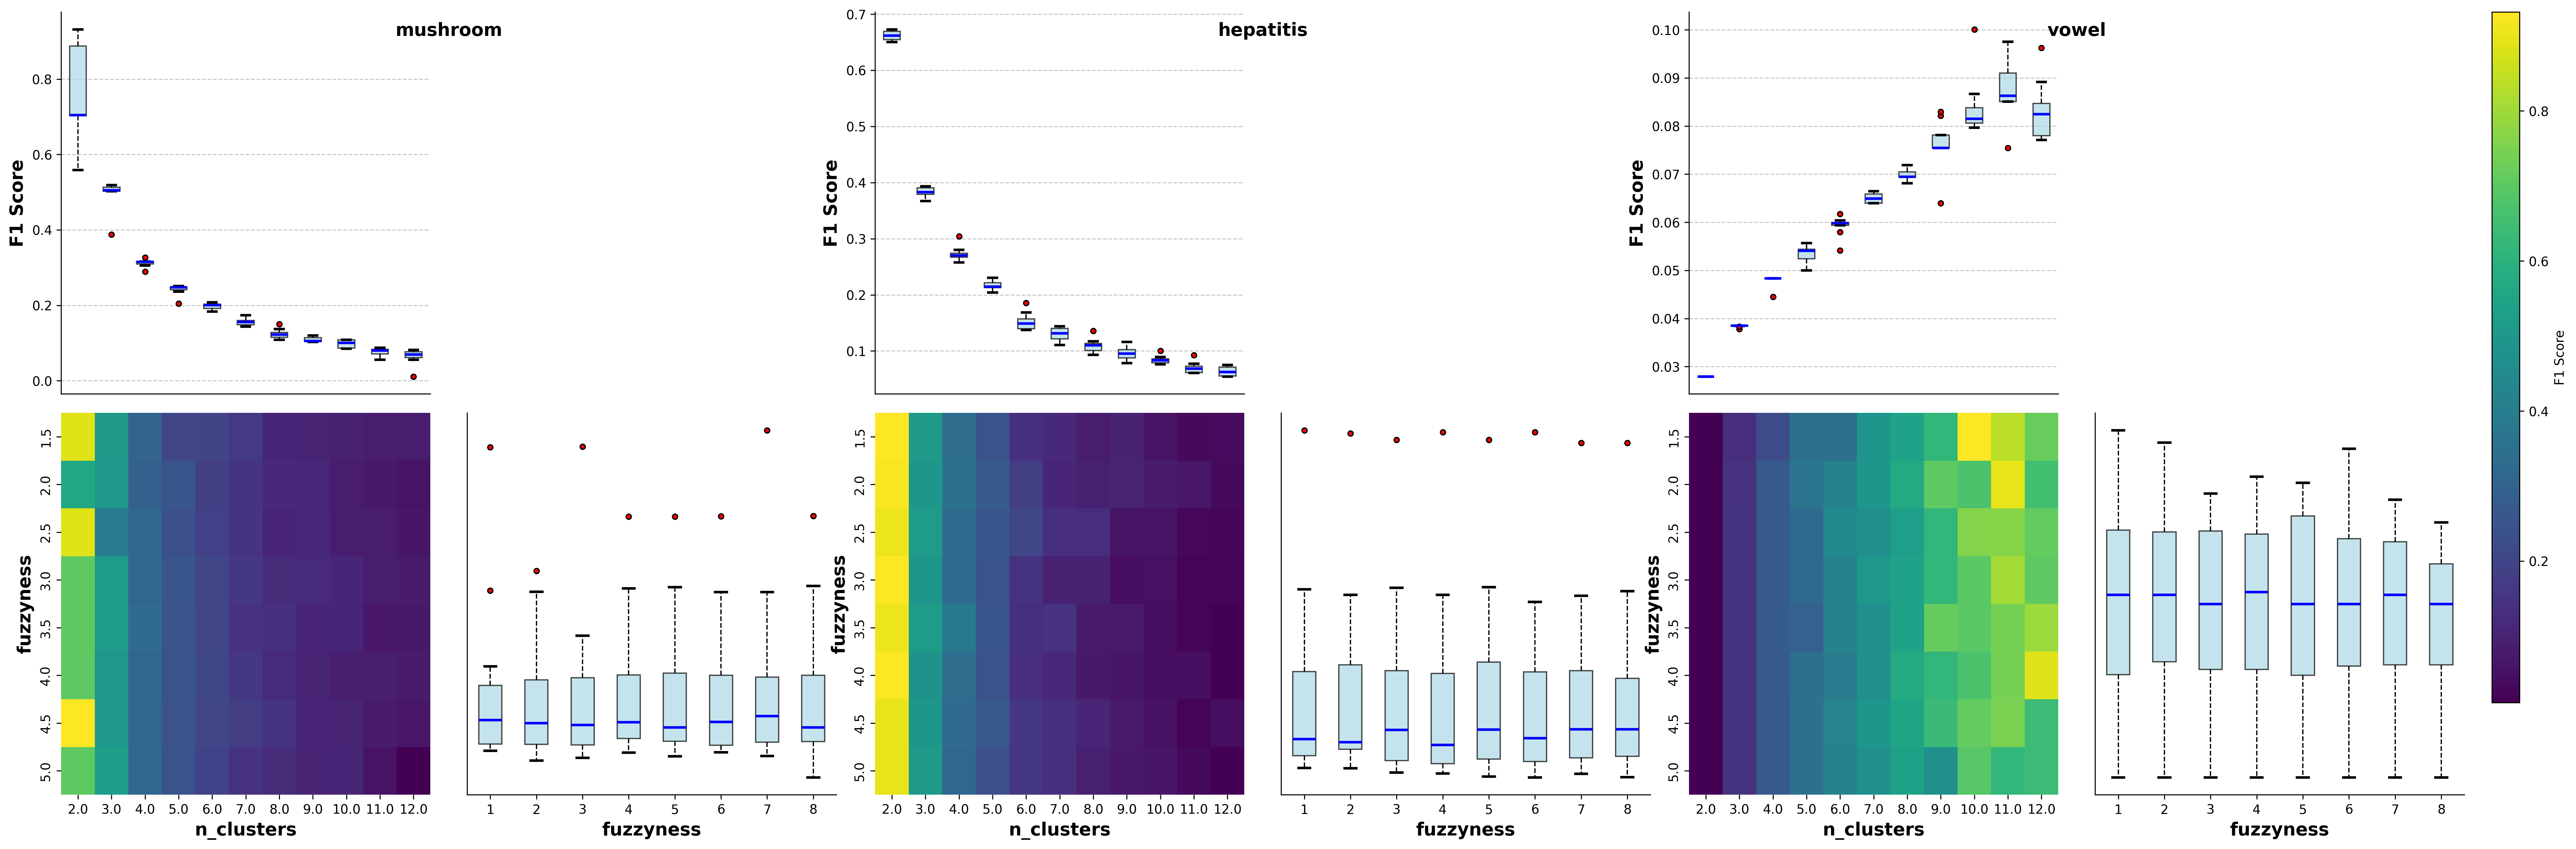
\includegraphics[width=0.5\textwidth]{figures/interactions_fuzzy_cmeans.png}
    \caption{Parameter interactions for gs-FCM}
    \label{fig:interactions_gsfcm}
\end{figure}


Figure~\ref{fig:interactions_gsfcm} presents the interaction effects between the key parameters of the Fuzzy C-Means clustering algorithm, namely the number of clusters ($n\_clusters$) and the fuzziness coefficient, across three datasets: \textit{hepatitis}, \textit{mushroom}, and \textit{vowel}. Each grid provides two types of visualizations: boxplots illustrating the variation in F1 score across different $n\_clusters$ values and heatmaps depicting the interaction between $n\_clusters$ and the fuzziness coefficient.

The boxplots indicate that, for all datasets, the performance of the clustering algorithm (measured in terms of F1 score) is sensitive to the choice of $n\_clusters$. For the \textit{hepatitis} dataset, the F1 score decreases steadily as the number of clusters increases, suggesting that simpler models (with fewer clusters) yield better results. This trend is less pronounced for the \textit{mushroom} dataset, where the F1 score stabilizes at a relatively high level as $n\_clusters$ increases. Conversely, the \textit{vowel} dataset demonstrates an improvement in F1 score with larger $n\_clusters$, indicating that more complex clustering structures are better suited for this dataset.

The heatmaps reveal nuanced interactions between $n\_clusters$ and the fuzziness parameter. For the \textit{hepatitis} dataset, lower values of fuzziness (closer to 1.5) combined with fewer clusters yield the highest F1 scores. This suggests that crisp clusters are more appropriate for this dataset. In contrast, for the \textit{mushroom} dataset, the heatmap indicates less sensitivity to the fuzziness parameter, as high F1 scores are maintained across a range of parameter combinations. The \textit{vowel} dataset, however, benefits from higher fuzziness values when paired with larger $n\_clusters$, suggesting that soft cluster boundaries improve performance for this dataset's characteristics.

Overall, the results highlight the importance of dataset-specific tuning of Fuzzy C-Means parameters. The \textit{hepatitis} dataset favors simple models with low fuzziness and fewer clusters, while the \textit{vowel} dataset benefits from greater complexity in terms of both parameters. The \textit{mushroom} dataset demonstrates robustness across a wider range of parameter combinations, underscoring its relative insensitivity to these hyperparameters.

These findings emphasize the need for careful hyperparameter optimization and underscore the variability of clustering behavior across datasets with differing characteristics.

